\documentclass[12pt]{article}  % 官方要求字号不小于 12 号,此处选择 12 号字体

% 本模板不需要填写年份,以当前电脑时间自动生成
% 请在以下的方括号中填写队伍控制号
\usepackage[UTF8]{ctex}
\usepackage{float}
\usepackage{algorithm}
\usepackage{algorithmic}
\usepackage[2510625]{easymcm}  % 载入 EasyMCM 模板文件
\problem{B}  % 请在此处填写题号
% \usepackage{mathptmx}  % 这是 Times 字体,中规中矩 
\usepackage{mathpazo}  % 这是 COMAP 官方杂志采用的更好看的 Palatino 字体,可替代以上的 mathptmx 宏包

\title{An MCM Paper Made by Team 2510625}  % 标题

% 如需要修改题头(默认为 MCM/ICM),请使用以下命令(此处修改为 MCM)
%\renewcommand{\contest}{MCM}

% 文档开始
\begin{document}

% 此处填写摘要内容
\begin{abstract}
    Here is the abstract of your paper.

    \textbf{对于问题1},我们仔细分析了旅客人数,税收的变化,财政在基建方面的投入比例对于政府最后的收入,环境质量以及社会满意度所产生的影响后进行了线性规划,建立了混合优化模型并用种群迭代机制从局部最优解找到了全局的最优解。基于往年朱诺的居民满意度调查数据和相对应年的游客数量对社会满意度和游客人数进行了一个非线性的拟合,其可靠度为0.7423。我们将社会满意度和环境质量通过乘以一个合适的系数进行了去量纲处理,方便衡量对目标函数的影响。根据我们的模型生成的结果显示在游客人数为1552632,游客税率为8\%,废物管理投入占比为0.128,水资源管理投入占比为0.113,环境保护投入占比为0.159的时候,总收入为295000000000美元,$CO_{2}$的排放量为285684.21吨,居民满意度为65.84(100为最大),环境指数为0.5014(1为最大,越小越好)。敏感性分析上,我们分析了变量的局部敏感性和全局敏感性,具体结果如图x所示并得出人数是关键的变量。

    Secondly, that is ...

    Finally, that is ...

    % 美赛论文中无需注明关键字。若您一定要使用,
    % 请将以下两行的注释号 '%' 去除,以使其生效
    % \vspace{5pt}
    % \textbf{Keywords}: MATLAB, mathematics, LaTeX.

\end{abstract}

\maketitle  % 生成 Summary Sheet
\tableofcontents  % 生成目录


% 正文开始
\section{Introduction}
\subsection{Problem Background}
Here is the problem background. Three major problems are discussed in this paper, which are:
\begin{itemize}
    \item \textbf{地理位置:}朱诺市是美国阿拉斯加州的首府,位于阿拉斯加东南部,拥有约30,000名居民。这座城市以其丰富的自然资源、独特的地理位置和迷人的自然景观而闻名,是许多游客前往阿拉斯加的首选目的地之一。朱诺市不仅是阿拉斯加的政治中心,也是一个重要的旅游枢纽,以其冰川、雨林和丰富的野生动物资源吸引着来自世界各地的游客。
    \item \textbf{旅游现状:}近年来,朱诺市的旅游业经历了迅猛的发展,尤其是在邮轮旅游方面。2023年,朱诺市创下了接待160万邮轮游客的纪录,单日最多接待7艘大型邮轮,游客数量高达20,000人。\cite{1}这些游客为城市带来了可观的经济收益,约3.75亿美元。\cite{2}然而,这种快速发展的旅游业也带来了一系列问题,尤其是与过度旅游相关的挑战。
    \item \textbf{环境影响:}朱诺市的门登霍尔冰川是该市的主要旅游景点之一,但近年来由于气温上升,冰川正在快速消退。自2007年以来,冰川已经后退了相当于八个足球场的距离。这种环境变化不仅对自然景观造成了破坏,也引发了当地居民对旅游业可持续性的担忧。\cite{3}
\end{itemize}

\begin{figure}[H]
	\centering
	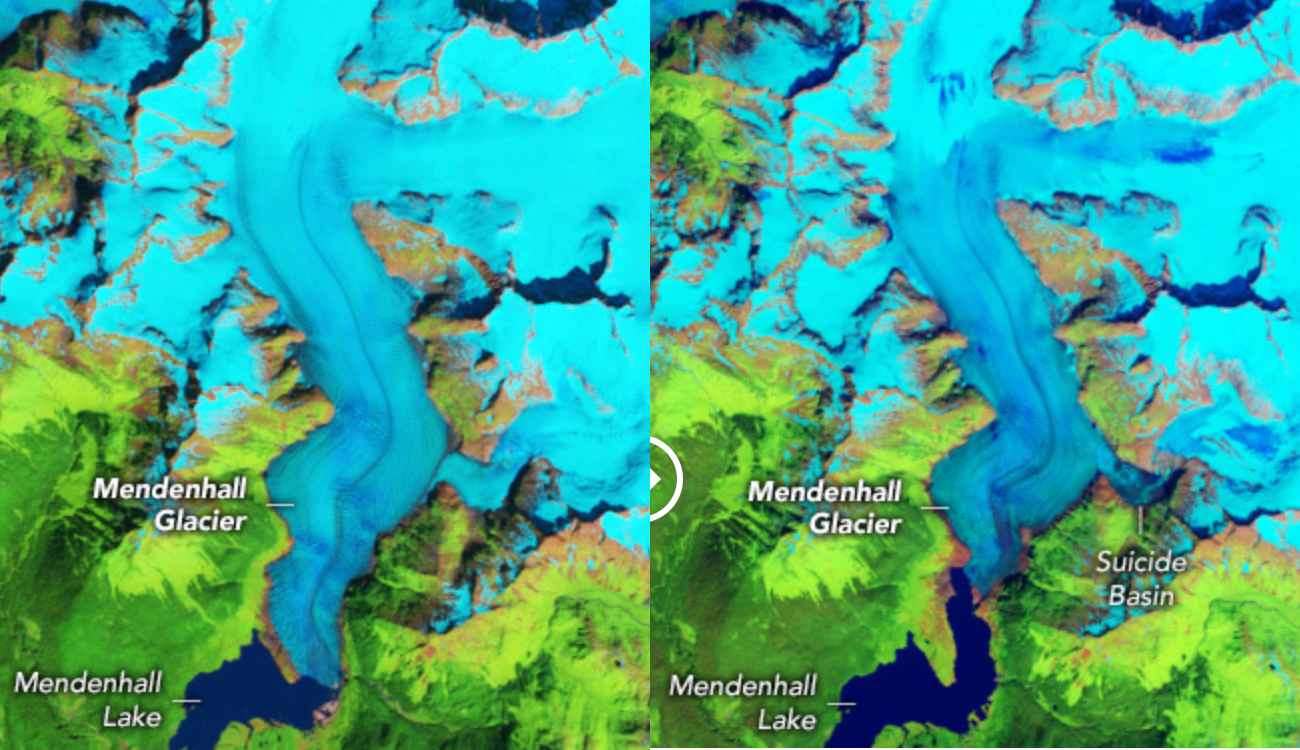
\includegraphics[width=.8\textwidth]{glacier.png}
	\caption{glacier}\label{fig:glacier}
\end{figure}

\subsection{Problem Restatement and Analysis}
\begin{itemize}
    \item \textbf{Problem1: }建立一个可持续旅游产业的模型,它应当满足最大化收入,最大化环境质量且最大化社会满意度并对其进行敏感性分析。
    \item \textbf{Problem2: }建立一个模型去解决游客分流到其他人流量比较小的景点,这也是增加收入减少区域压力的措施。
    \item \textbf{Problem3: }展示模型如何可以适应另一个受过度旅游影响的旅游目的地,应当去获取另一个城市的相关信息并用模型进行预测。
    \item \textbf{Problem4: }展示模型随着具体措施会发生的变化以此来为决策者提供更好的建议,比如加酒店税、游客费用、每日游客数量上限以及限制酒精销售和消费等。
    \item \textbf{An article: }为朱诺市旅游局写一封一页的备忘录,概述结果的预测、各种措施的影响以及对如何优化结果的建议。
\end{itemize}

\subsection{Our work}
To avoid complicated description , intuitively reflect our work process, the flow chart is show
as the following figure:
\begin{figure}[H]
	\centering
	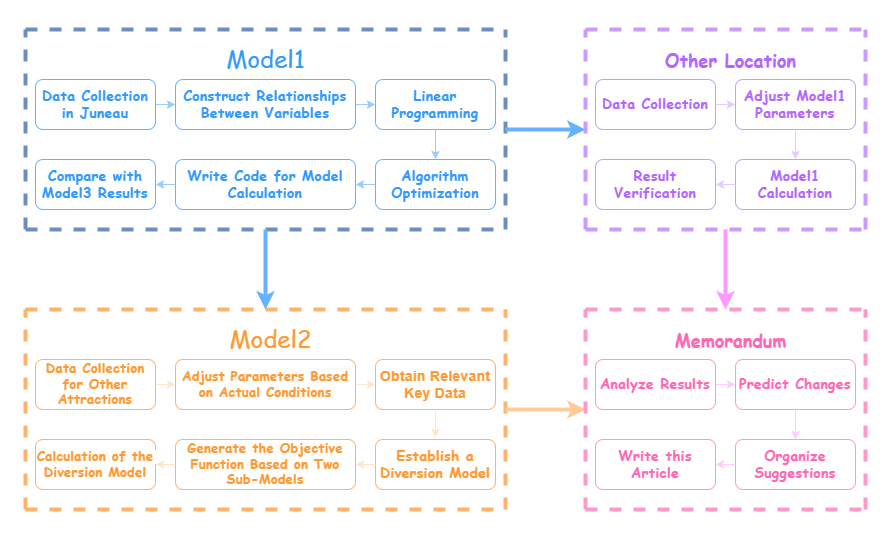
\includegraphics[width=\textwidth]{Process-map.png}
	\caption{Pcocess map}\label{fig:Process-map}
\end{figure}

\section{Preparation of the Models}
\subsection{Assumptions}

\subsection{Notations}
The primary notations used in this paper are listed in Table \ref{tb:notation}.

% 三线表示例
\begin{table}[H]
\begin{center}
\caption{Notations}
\begin{tabular}{>{\centering\arraybackslash}m{4cm} >{\centering\arraybackslash}m{10cm}}
	\toprule
		Symbol & Definition \\
	\midrule
	    \(R_{e}\) & Total tourism income \\
		\(N_{t}\) & Number of tourists \\
		\(N_{tmax}\) & Maximum number of tourists allowed per day \\
		\(\tau_{t}\) & Tax rate \\
		\(P_{t}\) & Average spending per tourist \\
		\(E\) & Environmental quality index \\
		\(CO_{2p}\) & Carbon emissions per person \\
		\(C_{base}\) & Base carbon emission treatment capacity \\
		\(C_{waste}\) & The amount of basic waste that the city can handle \\
		\(C_{water}\) & The basic amount of water that the city can provide \\
		\(S_{residents}\) & Residential satisfaction \\
		\(S\) & Social satisfaction \\
		\(P_{waste}\) & Cities' investment in waste management \\
		\(P_{water}\) & Cities' investment in water management \\
		\(P_{e}\) & Cities' investment in environment management \\
		\(Z\) & Representation of target equation\\
	\bottomrule
\end{tabular}\label{tb:notation}
\end{center}
\end{table}

\section{Solution to Problem1}
\subsection{建立一个可持续旅游发展的模型}
\subsubsection{找到状态变量之间的关系}
我们的目标函数应受收入,社会满意度和环境质量三者影响,若收入增加,则目标函数也应该增加,社会满意度同理,而环境质量越大负面影响也越大所以目标函数应减小,因此我们可以得到:
\begin{equation}
	Target\; equation:Z=R_e+S-E
\end{equation}

旅游的总收入应当和旅客的人数成简单的线性关系,因此我们可以很简单的得到公式2
\begin{equation}
    R_{e}(N_{t},P_{t}) = P_{t}N_{t}
\end{equation}

环境质量方面,主要考虑三个因素的影响:二氧化碳排放量,水的消耗量以及废物的产生量,而这三个因素都与游客人数密切相关。通过朱诺市的对这三个因子的处理能力和人均消耗/产生量,可以计算出朱诺市可以承载的人数$C_{base}$, $C_{waste}$, $C_{water}$,我们将实际的人数和承载人数相比,通过比例衡量体系压力。最后使用Analytic Hierarchy Process(ATP)方法结合各因子的重要性因素得到了公式3:
\begin{equation}
	E=k_{1}(CO_{2p}N_{t}-C_{base})+k_{2}\frac{N_{t}}{C_{waste}}+k_{3}\frac{N_{t}}{C_{water}}
\end{equation}

社会满意度方面,我们收集了朱诺市1998,2002,2006,2022,2023五年的社会满意度调查\cite{4},并摒除其无影响和不知道的无效评价,将剩下的评价依据李斯特量表分成了五级,并进行了量化以使结果保持在1以内。同时我们查找了这五年的游客人数\cite{5}来和社会满意度进行了数据拟合并得到了如下结果:
\begin{figure}[H]
	\centering
	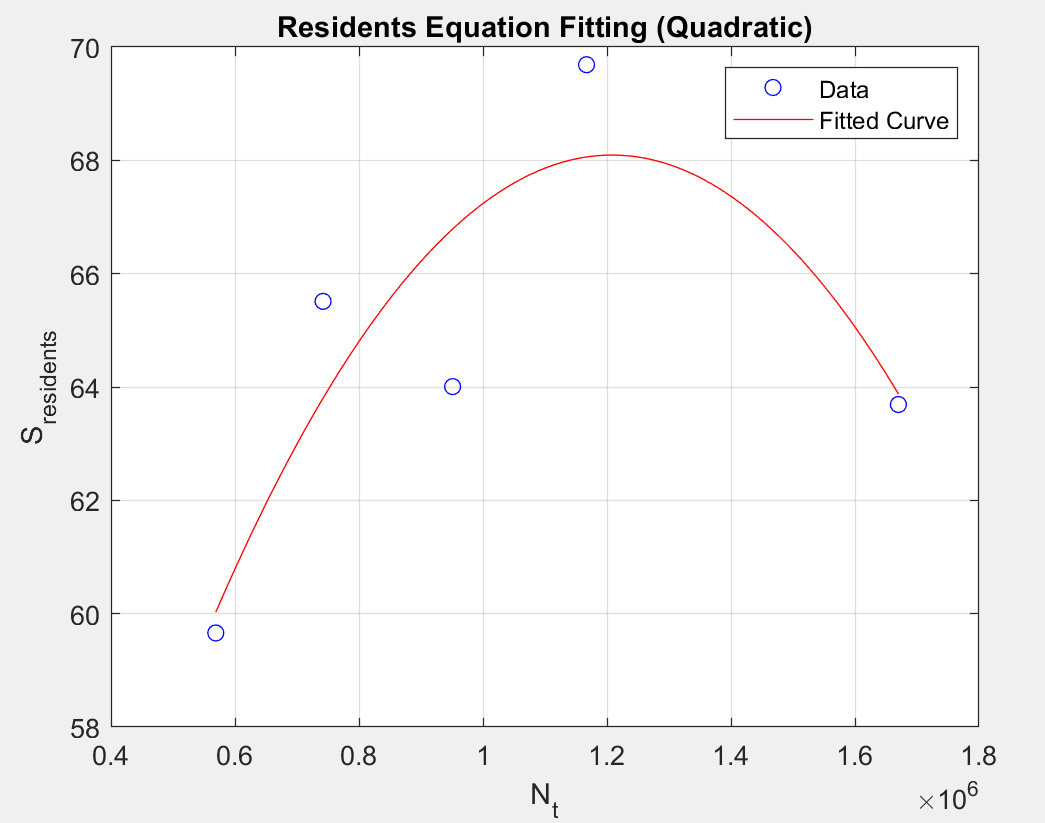
\includegraphics[width=.8\textwidth]{satisfaction.png}
	\caption{satisfaction}\label{fig:satisfaction}
\end{figure}
其中,$a_1 = -1.9753 \mathrm{e}{-11}$, $a_2 = 4.772\mathrm{e}{-5}$, $b = 39.2660$, $R^2 = 0.7423$。最后,为了消除量纲带来的影响以来衡量社会满意度对目标函数的影响,我们给数据加上了一个合适的系数$k4$。得到的公式4如下:
\begin{equation}
	\begin{cases}
		S_{residents}=a_{1}N_{t}^2+a_{2}N_{t} + b_{1} \\
		S=k_{4}S_{residents}
	\end{cases}
\end{equation}


	\begin{equation}
	\begin{cases}
		\frac{\mathrm{d}C_{waste}}{\mathrm{d}t}=\alpha_1P_{waste} \\
		\frac{\mathrm{d}C_{water}}{\mathrm{d}t}=\alpha_2P_{water} \\
		\frac{\mathrm{d}C_{base}}{\mathrm{d}t}=\alpha_3P_e \\
	\end{cases}
	\end{equation}

基建的额外投入方面,由于税率变化后的数据不够用于进行拟合以及考虑到税收对游客数量和消费意愿的抑制效应以及对消费的增长效应,结合实际已有的数据,认为在一定范围内波动时游客消费不受影响,简化为常数考虑。最后结合基建投入在政府实际分配中的比值,限定上限进行约束后得到公式6如下:
\begin{equation}
	\begin{cases}
		P_{waste} = k_5\tau_tR_e\\
		P_{water} = k_6\tau_tR_e\\
		P_{e}=k_7\tau_{t}R_e \\
		k_5+k_6+k_7 \leqslant 0.4
	\end{cases}
\end{equation}
\subsubsection{找到约束条件}
在经济方面,很显然我们有$R_e$必须要大于等于0。为了限制税率的值,我们根据xxx得出税率应小于等于8\%。因此有公式7:
\begin{equation}
	Financial:
	\begin{cases}
		R_{e}\geqslant 0 \\
		\tau_{t}\leqslant 8\% \\
	\end{cases}
\end{equation}

游客人数方面,我们依据朱诺市的政策\cite{6}得出了每天的游客的人数限制。公式8如下:
\begin{equation}
	Tourism:
		0\leqslant N_{t}\leqslant N_{tmax}\\
\end{equation}

环境方面,以NASA的冰川融化数据\cite{7}为基础,通过度日因子法来进行量化计算,最后通过二氧化碳影响温度进而影响速度的因素来限定了二氧化碳的最大排放量。而在水资源最大承载量和废物处理最大承载量上面,考虑到旺季人数占全年的比例以及对于基建的压力,升大设置1.2倍日平均承载量作为上限来限制人数。公式9如下:
\begin{equation}
	Environmental:
	\begin{cases}
		N_{t}\cdot CO_{2p}\leqslant CO_{2max} \\
		0.012N_t\leqslant \frac{1.2}{365}C_{waste} \\
		0.012N_t\leqslant \frac{1.2}{365}C_{water}
	\end{cases}
\end{equation}

社会满意度方面,经过合适的量化后,我们将60作为及格线。故公式10如下:
\begin{equation}
	Societal:\ S_{residents} \geqslant 60
\end{equation}	
\subsubsection{多起点的混合优化策略}
由于我们的模型共有五个决策变量,分别是\(N_t\),\(\tau_t\),\(k_5\),\(k_6\),\(k_7\),他们之间相互影响且对目标函数不同程度的影响。为了在每个决策变量在局部达到相对较优的条件下,尽可能使全局目标达到最佳,包括旅游收入最高,环境影响最小和居民满意度最高等等,我们使用多起点的混合优化策略来对目标函数的各个影响因子进行优化,其伪代码如下:
\begin{algorithm}
	\caption{Multi-start Optimization Algorithm}
	\begin{algorithmic}[1]
		\STATE \textbf{Input:} $n\_starts,\ Nmax,\ objective\_function$
		\STATE \textbf{Output:} $best\_result$
		\vspace{0.2cm}
		\STATE /* Initialize variables*/
		\STATE $best\_result\leftarrow null$
		\STATE $best\_objective\leftarrow \infty$
		\STATE /* Generate starting points for each parameter */
		\STATE $Nt\_starts\leftarrow linspace(100000,\,0.8\times Nmax,\,n\_starts)$
		\STATE $\tau\_starts\leftarrow linspace(0.02,\,0.07,\,n\_starts)$
		\STATE $k\_starts\leftarrow linspace(0.05,\,0.15,\,n\_starts)$
		\vspace{0.2cm}
		\STATE \textbf{Define optimization bounds}
		\vspace{0.2cm}
		\STATE /* Perform optimization from multiple starting points */
		\FOR{$i\leftarrow 0$ \TO $n\_starts-1$}
		\STATE /* Construct initial point */
		\STATE $x0\leftarrow [Nt\_starts[i],\ \tau\_starts[i],\ k\_starts[i],\ k\_starts[i]]$
		\STATE /* Minimize objective function */
		\STATE $result\leftarrow \textbf{minimize\_function}$
		\STATE /* Update best result if better solution found */
		\IF{$result.success$ \AND $result.objective\ <\ best\_objective$}
		\STATE $best\_objective\leftarrow result.objective$
		\STATE $best\_result\leftarrow deepcopy(result)$
		\ENDIF
		\ENDFOR
		\vspace{0.2cm}
		\RETURN $best\_result$
	\end{algorithmic}
\end{algorithm}

模型的解决方案和输出: 模型通过对多个影响因素进行多起点优化,最终得到最佳优化情况。
\subsubsection{计算结果}
$CO_{2max}$的计算过程,$C_{waste}$和$C_{water}$的计算过程。

旅游总收入上,根据以往的数据,我们给旅客平均消费值赋值为x。经过我们的计算可以得到游客每年人数应为x人,$P_e$为x,结合以往的数据来看,这个数据是相对合理的。

居民满意度上,将旅客人数带进拟合方程后可以得到居民满意度为x,符合我们的预期范围。

环境质量上,经过我们的ATP法得出$k1 = X$, $k2 = X$, $k3 = X$,将旅游人数和$CO_{2max}$, $C_{waste}$,$C_{water}$, $N_t$带入方程后得出结果为x,符合我们的预期范围。
\subsection{敏感度分析}
因为我们使用了混合优化策略,故我们同时分析了输入变量$N_t$, $\tau _t$, $k5$, $k6$, $k7$的局部敏感度和全局敏感性,代码如下:
\begin{algorithm}
	\caption{$Sensitive Analysis$}
	\begin{algorithmic}[1]
		\STATE Initialize variables
		\FOR{each element in the list}
			\IF{condition is met}
				\STATE Perform action
			\ELSE
				\STATE Perform another action
			\ENDIF
		\ENDFOR
		\STATE Return result
	\end{algorithmic}
\end{algorithm}

结果如下图所示:
\begin{figure}[H]
	\centering
	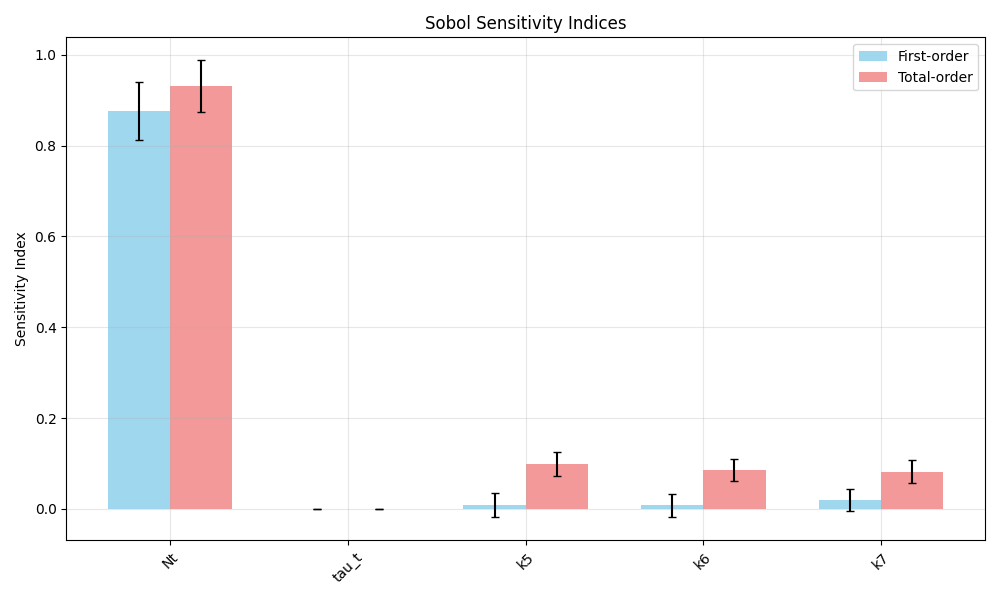
\includegraphics[width=.8\textwidth]{sensitive.png}
	\caption{Sensitive Analysis}\label{fig:sensitive}
\end{figure}

通过图片我们不难看出,旅客人数为关键的变量,其在局部和全局中的敏感性分别达到了x和x,远大于其他的输入变量,而这也符合朱诺市作为一个旅游城市收入受旅客人数影响较大的客观事实。
\section{Solution to Problem2}
\subsection{建立分流模型}

\subsection{Commetary on Model 2}
The instance of long and wide tables are shown in Table \ref{tb:longtable}.

% 长表格示例,更多用法请参考 longtable 宏包文档
% 以下环境及对应参数可实现表格内的自动换行与表格的自动断页
% 您也可以选择自行载入 tabularx 宏包,并通过 X 参数指定对应列自动换行
\begin{longtable}{ p{4em} p{14em} p{14em} }
\caption{Basic Information about Three Main Continents (scratched from Wikipedia)}
\label{tb:longtable}\\
\toprule
Continent & Description & Information \\
\midrule
Africa & Africa Continent is surrounded by the Mediterranean Sea to the
north, the Isthmus of Suez and the Red Sea to the northeast, the Indian
Ocean to the southeast and the Atlantic Ocean to the west. &
At about 30.3 million km$^2$ including adjacent islands, it covers 6\%
of Earth's total surface area and 20\% of its land area. With 1.3
billion people as of 2018, it accounts for about 16\% of the world's
human population. \\
\midrule
Asia & Asia is Earth's largest and most populous continent which
located primarily in the Eastern and Northern Hemispheres.
It shares the continental landmass of Eurasia with the continent
of Europe and the continental landmass of Afro-Eurasia with both
Europe and Africa. &
Asia covers an area of 44,579,000 square kilometres, about 30\%
of Earth's total land area and 8.7\% of the Earth's total surface
area. Its 4.5 billion people (as of June 2019) constitute roughly
60\% of the world's population. \\
\midrule
Europe & Europe is a continent located entirely in the Northern
Hemisphere and mostly in the Eastern Hemisphere. It comprises the
westernmost part of Eurasia and is bordered by the Arctic Ocean to
the north, the Atlantic Ocean to the west, the Mediterranean Sea to
the south, and Asia to the east. &
Europe covers about 10,180,000 km$^2$, or 2\% of the Earth's surface
(6.8\% of land area), making it the second smallest
continent. Europe had a total population of about 741 million (about
11\% of the world population) as of 2018. \\
\bottomrule
\end{longtable}

Figure \ref{fig:subfigures} gives an example of subfigures. Figure \ref{subfig:left} is on the left, and Figure \ref{subfig:right} is on the right.

% 子图(多图并列)示例,更多用法请参考 subfigure 宏包文档
% 如果您只希望几张图并列,不需要额外的 caption,那么在 figure 环境中
% 连续插入总宽度不超过 \textwidth 的多个 \includegraphics 命令即可
\begin{figure}[htbp]
\centering
\begin{subfigure}[b]{.4\textwidth}
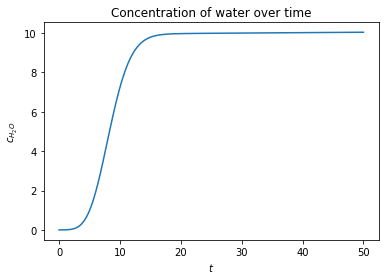
\includegraphics[width=\textwidth]{water.png}
\caption{Image on the left}\label{subfig:left}
\end{subfigure}
\begin{subfigure}[b]{.4\textwidth}
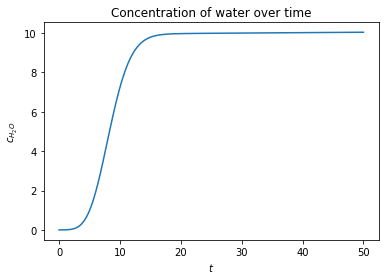
\includegraphics[width=\textwidth]{water.png}
\caption{Image on the right}\label{subfig:right}
\end{subfigure}
\caption{Two images}\label{fig:subfigures}
\end{figure}

\section{Solution to Problem3}
为了展示模型是如何适应另一个受过度旅游影响的,我们经过数据的查找和收集决定选择位于中国四川省的九寨沟风景区来进行分析。

因为每个地方的基础设施压力,人均消费等都大不相同,我们需要经过数据调研修改相应的参数后才能使用当前的模型进行预测。

通过对官网数据的收集\cite{8},我们可以得出九寨沟县每年的收入和九寨沟风景区之间的关系。但是由于官方网站缺乏相应的满意度调查等信息,我们根据社会上的普遍评价对这些值进行了简单的估计,通过修改相应的限制条件,如水资源的人均消耗量,废物的人均产生量,水资源和废物处理的承载能力,游客人均消费水平,我们可以将模型适用于九寨沟的情况。根据我们模型跑出来的结果显示,xxx。这些数据和往年相比具有合理性,符合实际的基本预期。


% 以下为信件/备忘录部分,不需要可自行去掉
% 如有需要可将整个 letter 环境移动到文章开头或中间
% 请在第二个花括号内填写标题,如「信件」(Letter)或「备忘录」(Memorandum)
\begin{letter}{Memorandum}
\begin{flushleft}  % 左对齐环境,无首行缩进
\textbf{To:} 朱诺市政府\\
\textbf{From:} Team 2510625\\
\textbf{Date:} January 27th, 2025\\
\textbf{Subject:} 关于政府在旅游业上的一些建议
\end{flushleft}

随着旅游市场的不断发展,朱诺市作为阿拉斯加的首府,拥有丰富的自然景观和独特的文化魅力,吸引了大量游客前来观光旅游。为了更好地了解旅游市场的发展趋势,评估各种措施对旅游市场的影响,并提出优化建议,我们进行了深入的市场调研和数据分析。

首先是关于旅游市场的预测,根据我们的市场调研和数据分析,预计未来几年朱诺市的旅游市场将呈现以下趋势:
\textbf{游客数量增长:}随着全球经济的复苏和人们生活水平的提高,预计未来几年朱诺市的游客数量将呈现稳步增长的趋势。特别是来自亚洲和欧洲的游客数量将有较大幅度的增加。
\textbf{旅游季节变化:}虽然夏季仍然是朱诺市的旅游旺季,但随着冬季旅游项目的不断丰富,如狗拉雪橇、冰钓等,冬季旅游市场也将逐渐升温。

二是各种措施的影响,为了促进朱诺市旅游市场的发展,我们分析了一系列措施,这些措施对旅游市场产生了以下影响:
\textbf{适量提高税率:}适量提高税率短时间不会对旅游人数产生较大的影响,而税率的提高可以增加旅游业带来的收入,额外收入增加后可以对基建投入更多的金钱以来提高水资源和废物处理承载能力。
\textbf{限制每日的游客人数:}限制每日的人数有助于缓解基础设施压力,提高居民满意度,同时如果限制的人数控制在一个比奥较好的值也能确保每日的收入保持在一个比较高的水平。

最后是一些优化的建议:
\textbf{加强旅游基础设施建设:}继续加大对旅游基础设施的投入,进一步改善住宿、餐饮、交通等方面的条件。特别是要加大对偏远地区的旅游基础设施建设,提高旅游的可达性和便利性。有利于游客参观更多的景点,分散个别热门景点的压力。
\textbf{提升旅游服务质量:}加强对旅游从业人员的培训,提高旅游服务的质量和水平。特别是要加强对导游、酒店服务人员等的培训,提高他们的专业素质和服务意识。这样可以提升朱诺市的旅游风评,增加游客前来的意愿。
\textbf{加强市场营销推广:}继续在国内外主要旅游市场进行市场营销推广,提高朱诺市的知名度和美誉度。可以通过举办旅游推介会、参加旅游展会等方式,向更多的游客宣传朱诺市的旅游资源和旅游产品以来吸引更多游客和刺激游客消费,提高游客平均消费水平。

\end{letter}


% 参考文献,此处以 MLA 引用格式为例

\begin{thebibliography}{99}
\bibitem{1} \url{https://abc7.com/post/juneau-alaska-cruise-ship-limits-overtourism/15048713/}
\bibitem{2} \url{https://juneau.org/wp-content/uploads/2024/01/CBJ-Cruise-Impacts-2023-Report-1.22.24.pdf}
\bibitem{3} \url{https://alaskapublic.org/2023/08/07/crammed-with-tourists-juneau-wonders-what-will-happen-as-mendenhall-glacier-recedes/}
\bibitem{4} \emph{A simple, easy \LaTeX\ template for MCM/ICM: EasyMCM}. (2018). Retrieved December 1, 2019, from\url{https://www.cnblogs.com/xjtu-blacksmith/p/easymcm.html}
\bibitem{7} \url{https://earthobservatory.nasa.gov/images/151682/alaskas-mendenhall-glacier}
\bibitem{8} \url{https://www.jiuzhai.com/news/number-of-tourists/}
\end{thebibliography}


% 以下为附录内容
% 如您的论文中不需要附录,请自行删除
\begin{subappendices}  % 附录环境

\section{Appendix A: Further on \LaTeX}
To clarify the importance of using \LaTeX\ in MCM or ICM, several points need to be covered, which are \ldots

To be more specific, \ldots

All in all, \ldots

Anyway, nobody \textbf{really} needs such appendix \ldots

\section{Appendix B: Program Codes}
Here are the program codes we used in our research.

% 代码环境示例三则
% 如您的论文不需要展示代码,请删除
% 更多用法,请参考 listings 宏包文档

% Python 代码示例


% MATLAB 代码示例
\begin{lstlisting}[language=MATLAB, name={test.m}]
% MATLAB code example
for i = 1:10
    disp("hello, world!");
end
\end{lstlisting}

% C++ 代码示例
\begin{lstlisting}[language=C++, name={test.cpp}]
// C++ code example
#include <iostream>
using namespace std;

int main() {
    for (int i = 0; i < 10; i++)
        cout << "hello, world" << endl;
    return 0;
}
\end{lstlisting}

\end{subappendices}  % 附录内容结束

\end{document}  % 结束
